\documentclass{article}
\usepackage{lmodern}
\usepackage[T1]{fontenc}
\usepackage{shapepar}
\usepackage{microtype}
\usepackage{lipsum}
\usepackage{pgfplots}
\pgfplotsset{compat=1.9}
\usepackage{tikz}
\usetikzlibrary{calc,fit,intersections,folding}
\usepackage{pstricks-add}
\usetikzlibrary{arrows.meta,angles,arrows,quotes,backgrounds}

\usepackage[a1paper, landscape]{geometry}

\newcommand{\tubecolor}{blue}
\newcommand{\thickness}{0.6mm}
\newcommand{\n}{3mm}


\newcommand{\tubing}[4]{
        \coordinate (1) at (0,0);
        \coordinate (2) at (1,1);
        \coordinate (3) at (1,-1);
        \coordinate (4) at (-1,-1);
        \coordinate (5) at (-1,1);

        
        %\foreach \n in {1,2,3,4,5}{\node (\n) at (\n) {$\n$};}
        \foreach \n in {2,3,4,5}{\draw[line width = 1mm] (1) -- (\n);}

        \foreach \n in {1,2,3,4,5}{\node[draw, shape=circle, fill=black, text=white] at (\n) {\Huge$\mathbf{\n}$};}
        

        
        %Tube 1234
        \begin{scope}[on background layer]
            \fill[\tubecolor] (#1) circle (\n + 9*\thickness);
            \fill[\tubecolor] (#2) circle (\n + 9*\thickness);
            \fill[\tubecolor] (#3) circle (\n + 9*\thickness);
            \fill[\tubecolor] (#4) circle (\n + 9*\thickness);
            \draw[\tubecolor] [line width = 4*(\n + 9*\thickness)] (#1.center) -- (#2.center);
            \draw[\tubecolor] [line width = 4*(\n + 9*\thickness)] (#1.center) -- (#3.center);
            \draw[\tubecolor] [line width = 4*(\n + 9*\thickness)] (#3.center) -- (#2.center);
            \draw[\tubecolor] [line width = 4*(\n + 9*\thickness)] (#1.center) -- (#4.center);
            \draw[\tubecolor] [line width = 4*(\n + 9*\thickness)] (#2.center) -- (#4.center);
            \draw[\tubecolor] [line width = 4*(\n + 9*\thickness)] (#3.center) -- (#4.center);
            
            \fill[white] (#1) circle (\n + 8*\thickness);
            \fill[white] (#2) circle (\n + 8*\thickness);
            \fill[white] (#3) circle (\n + 8*\thickness);
            \fill[white] (#4) circle (\n + 8*\thickness);
            \draw[white] [line width = 4*(\n + 8*\thickness)] (#1.center) -- (#2.center);
            \draw[white] [line width = 4*(\n + 8*\thickness)] (#1.center) -- (#3.center);
            \draw[white] [line width = 4*(\n + 8*\thickness)] (#3.center) -- (#2.center);
            \draw[white] [line width = 4*(\n + 8*\thickness)] (#1.center) -- (#4.center);
            \draw[white] [line width = 4*(\n + 8*\thickness)] (#2.center) -- (#4.center);
            \draw[white] [line width = 4*(\n + 8*\thickness)] (#3.center) -- (#4.center);
        \end{scope}
        %Tube 123
        \begin{scope}[on background layer]
            \fill[\tubecolor] (#1) circle (\n + 7*\thickness);
            \fill[\tubecolor] (#2) circle (\n + 7*\thickness);
            \fill[\tubecolor] (#3) circle (\n + 7*\thickness);
            \draw[\tubecolor] [line width = 4*(\n + 7*\thickness)] (#1.center) -- (#2.center);
            \draw[\tubecolor] [line width = 4*(\n + 7*\thickness)] (#1.center) -- (#3.center);
            \draw[\tubecolor] [line width = 4*(\n + 7*\thickness)] (#3.center) -- (#2.center);
            
            \fill[white] (#1) circle (\n + 6*\thickness);
            \fill[white] (#2) circle (\n + 6*\thickness);
            \fill[white] (#3) circle (\n + 6*\thickness);
            \draw[white] [line width = 4*(\n + 6*\thickness)] (#1.center) -- (#2.center);
            \draw[white] [line width = 4*(\n + 6*\thickness)] (#1.center) -- (#3.center);
            \draw[white] [line width = 4*(\n + 6*\thickness)] (#3.center) -- (#2.center);
        \end{scope}

        %Tube 12
        \begin{scope}[on background layer]
            \fill[\tubecolor] (#1) circle (\n + 5*\thickness);
            \fill[\tubecolor] (#2) circle (\n + 5*\thickness);
            \draw[\tubecolor] [line width = 4*(\n + 5*\thickness)] (#1.center) -- (#2.center);
            
            \fill[white] (#1) circle (\n + 4*\thickness);
            \fill[white] (#2) circle (\n + 4*\thickness);
            \draw[white] [line width = 4*(\n + 4*\thickness)] (#1.center) -- (#2.center);
        \end{scope}
        %Tube 1
        \begin{scope}[on background layer]
            \fill[\tubecolor] (#1) circle (\n + 3*\thickness);
            
            \fill[white] (#1) circle (\n + 2*\thickness);
        \end{scope}}


\begin{document}
\thispagestyle{empty}
\begin{center}
    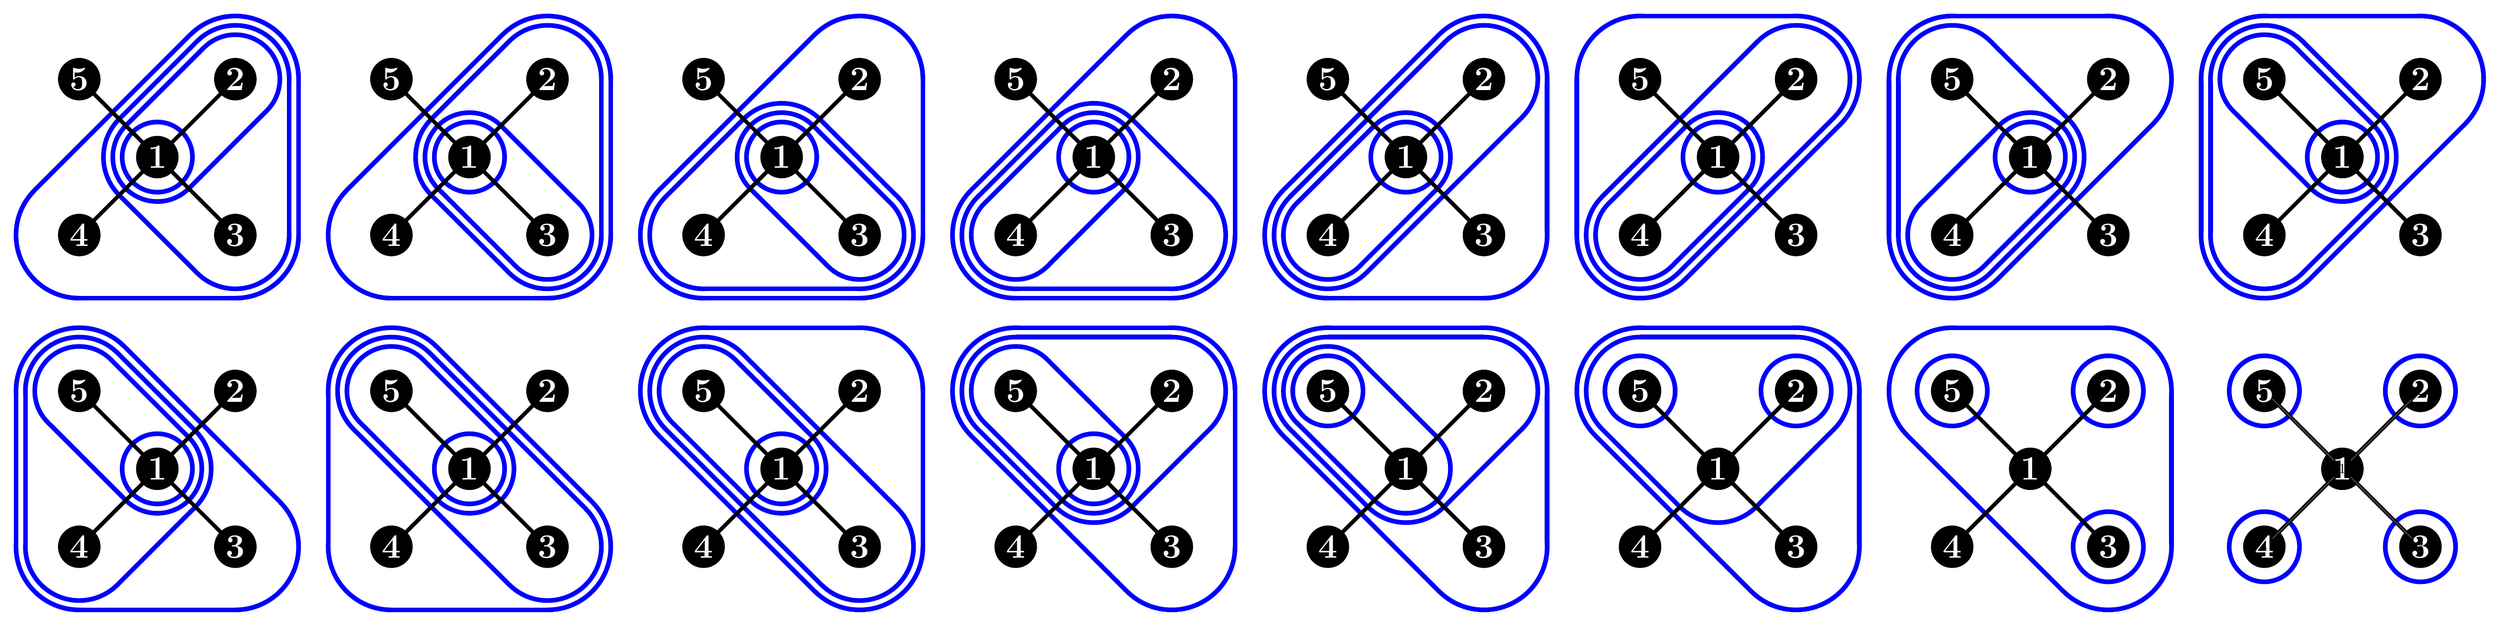
\begin{tikzpicture}[scale = 2]
    
    \begin{scope}[]
        \tubing{1}{2}{3}{4}
    \end{scope}
    \begin{scope}[xshift = 4cm]
        \tubing{1}{3}{2}{4}
    \end{scope}
    \begin{scope}[xshift = 8cm]
        \tubing{1}{3}{4}{2}
    \end{scope}
    \begin{scope}[xshift = 12cm]
        \tubing{1}{4}{3}{2}
    \end{scope}
    \begin{scope}[xshift = 16cm]
        \tubing{1}{4}{2}{3}
    \end{scope}
    \begin{scope}[xshift = 20cm]
        \tubing{1}{4}{2}{5}
    \end{scope}
    \begin{scope}[xshift = 24cm]
        \tubing{1}{4}{5}{2}
    \end{scope}
    \begin{scope}[xshift = 28cm, yshift = 0cm]
        \tubing{1}{5}{4}{2}
    \end{scope}
    \begin{scope}[xshift = 0cm, yshift = -4cm]
        \tubing{1}{5}{4}{3}
    \end{scope}
    \begin{scope}[xshift = 4cm, yshift = -4cm]
        \tubing{1}{5}{3}{4}
    \end{scope}
    \begin{scope}[xshift = 8cm, yshift = -4cm]
        \tubing{1}{5}{3}{2}
    \end{scope}
    \begin{scope}[xshift = 12cm, yshift = -4cm]
        \tubing{1}{5}{2}{3}
    \end{scope}

    \begin{scope}[xshift = 16cm, yshift = -4cm]
        
        \coordinate (1) at (0,0);
        \coordinate (2) at (1,1);
        \coordinate (3) at (1,-1);
        \coordinate (4) at (-1,-1);
        \coordinate (5) at (-1,1);

        
        %\foreach \n in {1,2,3,4,5}{\node (\n) at (\n) {$\n$};}
        \foreach \n in {2,3,4,5}{\draw[line width = 1mm] (1) -- (\n);}

        \foreach \n in {1,2,3,4,5}{\node[draw, shape=circle, fill=black, text=white] at (\n) {\Huge$\mathbf{\n}$};}
        
        %Tube 1235
        \begin{scope}[on background layer]
            \fill[\tubecolor] (1) circle (\n + 9*\thickness);
            \fill[\tubecolor] (2) circle (\n + 9*\thickness);
            \fill[\tubecolor] (3) circle (\n + 9*\thickness);
            \fill[\tubecolor] (5) circle (\n + 9*\thickness);
            \draw[\tubecolor] [line width = 4*(\n + 9*\thickness)] (1.center) -- (2.center);
            \draw[\tubecolor] [line width = 4*(\n + 9*\thickness)] (1.center) -- (3.center);
            \draw[\tubecolor] [line width = 4*(\n + 9*\thickness)] (3.center) -- (2.center);
            \draw[\tubecolor] [line width = 4*(\n + 9*\thickness)] (1.center) -- (5.center);
            \draw[\tubecolor] [line width = 4*(\n + 9*\thickness)] (2.center) -- (5.center);
            \draw[\tubecolor] [line width = 4*(\n + 9*\thickness)] (3.center) -- (5.center);
            
            \fill[white] (1) circle (\n + 8*\thickness);
            \fill[white] (2) circle (\n + 8*\thickness);
            \fill[white] (3) circle (\n + 8*\thickness);
            \fill[white] (5) circle (\n + 8*\thickness);
            \draw[white] [line width = 4*(\n + 8*\thickness)] (1.center) -- (2.center);
            \draw[white] [line width = 4*(\n + 8*\thickness)] (1.center) -- (3.center);
            \draw[white] [line width = 4*(\n + 8*\thickness)] (3.center) -- (2.center);
            \draw[white] [line width = 4*(\n + 8*\thickness)] (1.center) -- (5.center);
            \draw[white] [line width = 4*(\n + 8*\thickness)] (2.center) -- (5.center);
            \draw[white] [line width = 4*(\n + 8*\thickness)] (3.center) -- (5.center);
        \end{scope}
        %Tube 125
        \begin{scope}[on background layer]
            \fill[\tubecolor] (1) circle (\n + 7*\thickness);
            \fill[\tubecolor] (2) circle (\n + 7*\thickness);
            \fill[\tubecolor] (5) circle (\n + 7*\thickness);
            \draw[\tubecolor] [line width = 4*(\n + 7*\thickness)] (1.center) -- (2.center);
            \draw[\tubecolor] [line width = 4*(\n + 7*\thickness)] (1.center) -- (5.center);
            \draw[\tubecolor] [line width = 4*(\n + 7*\thickness)] (5.center) -- (2.center);
            
            \fill[white] (1) circle (\n + 6*\thickness);
            \fill[white] (2) circle (\n + 6*\thickness);
            \fill[white] (5) circle (\n + 6*\thickness);
            \draw[white] [line width = 4*(\n + 6*\thickness)] (1.center) -- (2.center);
            \draw[white] [line width = 4*(\n + 6*\thickness)] (1.center) -- (5.center);
            \draw[white] [line width = 4*(\n + 6*\thickness)] (5.center) -- (2.center);
        \end{scope}

        %Tube 15
        \begin{scope}[on background layer]
            \fill[\tubecolor] (1) circle (\n + 5*\thickness);
            \fill[\tubecolor] (5) circle (\n + 5*\thickness);
            \draw[\tubecolor] [line width = 4*(\n + 5*\thickness)] (1.center) -- (5.center);
            
            \fill[white] (1) circle (\n + 4*\thickness);
            \fill[white] (5) circle (\n + 4*\thickness);
            \draw[white] [line width = 4*(\n + 4*\thickness)] (1.center) -- (5.center);
        \end{scope} 
        %Tube 5
        \begin{scope}[on background layer]
            \fill[\tubecolor] (5) circle (\n + 3*\thickness);
            
            \fill[white] (5) circle (\n + 2*\thickness);
        \end{scope}
    \end{scope}
    
    \begin{scope}[xshift = 20cm, yshift = -4cm]
        
        \coordinate (1) at (0,0);
        \coordinate (2) at (1,1);
        \coordinate (3) at (1,-1);
        \coordinate (4) at (-1,-1);
        \coordinate (5) at (-1,1);

        
        %\foreach \n in {1,2,3,4,5}{\node (\n) at (\n) {$\n$};}
        \foreach \n in {2,3,4,5}{\draw[line width = 1mm] (1) -- (\n);}

        \foreach \n in {1,2,3,4,5}{\node[draw, shape=circle, fill=black, text=white] at (\n) {\Huge$\mathbf{\n}$};}
        
        %Tube 1235
        \begin{scope}[on background layer]
            \fill[\tubecolor] (1) circle (\n + 9*\thickness);
            \fill[\tubecolor] (2) circle (\n + 9*\thickness);
            \fill[\tubecolor] (3) circle (\n + 9*\thickness);
            \fill[\tubecolor] (5) circle (\n + 9*\thickness);
            \draw[\tubecolor] [line width = 4*(\n + 9*\thickness)] (1.center) -- (2.center);
            \draw[\tubecolor] [line width = 4*(\n + 9*\thickness)] (1.center) -- (3.center);
            \draw[\tubecolor] [line width = 4*(\n + 9*\thickness)] (3.center) -- (2.center);
            \draw[\tubecolor] [line width = 4*(\n + 9*\thickness)] (1.center) -- (5.center);
            \draw[\tubecolor] [line width = 4*(\n + 9*\thickness)] (2.center) -- (5.center);
            \draw[\tubecolor] [line width = 4*(\n + 9*\thickness)] (3.center) -- (5.center);
            
            \fill[white] (1) circle (\n + 8*\thickness);
            \fill[white] (2) circle (\n + 8*\thickness);
            \fill[white] (3) circle (\n + 8*\thickness);
            \fill[white] (5) circle (\n + 8*\thickness);
            \draw[white] [line width = 4*(\n + 8*\thickness)] (1.center) -- (2.center);
            \draw[white] [line width = 4*(\n + 8*\thickness)] (1.center) -- (3.center);
            \draw[white] [line width = 4*(\n + 8*\thickness)] (3.center) -- (2.center);
            \draw[white] [line width = 4*(\n + 8*\thickness)] (1.center) -- (5.center);
            \draw[white] [line width = 4*(\n + 8*\thickness)] (2.center) -- (5.center);
            \draw[white] [line width = 4*(\n + 8*\thickness)] (3.center) -- (5.center);
        \end{scope}
        %Tube 125
        \begin{scope}[on background layer]
            \fill[\tubecolor] (1) circle (\n + 7*\thickness);
            \fill[\tubecolor] (2) circle (\n + 7*\thickness);
            \fill[\tubecolor] (5) circle (\n + 7*\thickness);
            \draw[\tubecolor] [line width = 4*(\n + 7*\thickness)] (1.center) -- (2.center);
            \draw[\tubecolor] [line width = 4*(\n + 7*\thickness)] (1.center) -- (5.center);
            \draw[\tubecolor] [line width = 4*(\n + 7*\thickness)] (5.center) -- (2.center);
            
            \fill[white] (1) circle (\n + 6*\thickness);
            \fill[white] (2) circle (\n + 6*\thickness);
            \fill[white] (5) circle (\n + 6*\thickness);
            \draw[white] [line width = 4*(\n + 6*\thickness)] (1.center) -- (2.center);
            \draw[white] [line width = 4*(\n + 6*\thickness)] (1.center) -- (5.center);
            \draw[white] [line width = 4*(\n + 6*\thickness)] (5.center) -- (2.center);
        \end{scope}

        %Tube 2
        \begin{scope}[on background layer]
            \fill[\tubecolor] (2) circle (\n + 3*\thickness);
            
            \fill[white] (2) circle (\n + 2*\thickness);
        \end{scope} 
        %Tube 5
        \begin{scope}[on background layer]
            \fill[\tubecolor] (5) circle (\n + 3*\thickness);
            
            \fill[white] (5) circle (\n + 2*\thickness);
        \end{scope}
        
    \end{scope}
    
    \begin{scope}[xshift = 24cm, yshift = -4cm]
        
        \coordinate (1) at (0,0);
        \coordinate (2) at (1,1);
        \coordinate (3) at (1,-1);
        \coordinate (4) at (-1,-1);
        \coordinate (5) at (-1,1);

        
        %\foreach \n in {1,2,3,4,5}{\node (\n) at (\n) {$\n$};}
        \foreach \n in {2,3,4,5}{\draw[line width = 1mm] (1) -- (\n);}

        \foreach \n in {1,2,3,4,5}{\node[draw, shape=circle, fill=black, text=white] at (\n) {\Huge$\mathbf{\n}$};}
        
        %Tube 1235
        \begin{scope}[on background layer]
            \fill[\tubecolor] (1) circle (\n + 9*\thickness);
            \fill[\tubecolor] (2) circle (\n + 9*\thickness);
            \fill[\tubecolor] (3) circle (\n + 9*\thickness);
            \fill[\tubecolor] (5) circle (\n + 9*\thickness);
            \draw[\tubecolor] [line width = 4*(\n + 9*\thickness)] (1.center) -- (2.center);
            \draw[\tubecolor] [line width = 4*(\n + 9*\thickness)] (1.center) -- (3.center);
            \draw[\tubecolor] [line width = 4*(\n + 9*\thickness)] (3.center) -- (2.center);
            \draw[\tubecolor] [line width = 4*(\n + 9*\thickness)] (1.center) -- (5.center);
            \draw[\tubecolor] [line width = 4*(\n + 9*\thickness)] (2.center) -- (5.center);
            \draw[\tubecolor] [line width = 4*(\n + 9*\thickness)] (3.center) -- (5.center);
            
            \fill[white] (1) circle (\n + 8*\thickness);
            \fill[white] (2) circle (\n + 8*\thickness);
            \fill[white] (3) circle (\n + 8*\thickness);
            \fill[white] (5) circle (\n + 8*\thickness);
            \draw[white] [line width = 4*(\n + 8*\thickness)] (1.center) -- (2.center);
            \draw[white] [line width = 4*(\n + 8*\thickness)] (1.center) -- (3.center);
            \draw[white] [line width = 4*(\n + 8*\thickness)] (3.center) -- (2.center);
            \draw[white] [line width = 4*(\n + 8*\thickness)] (1.center) -- (5.center);
            \draw[white] [line width = 4*(\n + 8*\thickness)] (2.center) -- (5.center);
            \draw[white] [line width = 4*(\n + 8*\thickness)] (3.center) -- (5.center);
        \end{scope}

        %Tube 2
        \begin{scope}[on background layer]
            \fill[\tubecolor] (2) circle (\n + 3*\thickness);
            
            \fill[white] (2) circle (\n + 2*\thickness);
        \end{scope} 
        %Tube 5
        \begin{scope}[on background layer]
            \fill[\tubecolor] (5) circle (\n + 3*\thickness);
            
            \fill[white] (5) circle (\n + 2*\thickness);
        \end{scope}
        %Tube 3
        \begin{scope}[on background layer]
            \fill[\tubecolor] (3) circle (\n + 3*\thickness);
            
            \fill[white] (3) circle (\n + 2*\thickness);
        \end{scope}
    \end{scope}

    \begin{scope}[xshift = 28cm, yshift = -4cm]
        
        \coordinate (1) at (0,0);
        \coordinate (2) at (1,1);
        \coordinate (3) at (1,-1);
        \coordinate (4) at (-1,-1);
        \coordinate (5) at (-1,1);

        
        %\foreach \n in {1,2,3,4,5}{\node (\n) at (\n) {$\n$};}
        \foreach \n in {2,3,4,5}{\draw[line width = 1mm] (1) -- (\n);}

        \foreach \n in {1,2,3,4,5}{\node[draw, shape=circle, fill=black, text=white] at (\n) {\Huge$\mathbf{\n}$};}
        

        \foreach \n in {1,2,3,4,5}{\node (\n) at (\n) {$\n$};}
        \foreach \n in {2,3,4,5}{\draw[gray] (1) -- (\n);}

        %Tube 2
        \begin{scope}[on background layer]
            \fill[\tubecolor] (2) circle (\n + 3*\thickness);
            
            \fill[white] (2) circle (\n + 2*\thickness);
        \end{scope} 
        %Tube 5
        \begin{scope}[on background layer]
            \fill[\tubecolor] (5) circle (\n + 3*\thickness);
            
            \fill[white] (5) circle (\n + 2*\thickness);
        \end{scope}
        %Tube 3
        \begin{scope}[on background layer]
            \fill[\tubecolor] (3) circle (\n + 3*\thickness);
            
            \fill[white] (3) circle (\n + 2*\thickness);
        \end{scope}
        \begin{scope}[on background layer]
            \fill[\tubecolor] (4) circle (\n + 3*\thickness);
            
            \fill[white] (4) circle (\n + 2*\thickness);
        \end{scope}
    \end{scope}

    \end{tikzpicture}
\end{center}
\end{document}